%!TEX root = ../tommaso-thesis.tex
%!TEX spellcheck = en_US


%\documentclass[conference]{IEEEtran}

\usepackage{xspace,graphicx,url,paralist} % ,hyperref}

\usepackage{xcolor,colortbl}

% status color definition
\definecolor{active}{HTML}{FF6600}
\definecolor{work needed}{HTML}{FF0000}
\definecolor{closed}{HTML}{888888}
\definecolor{resolved}{HTML}{666666}
\definecolor{unknown}{HTML}{D3D3D3}

\newcommand{\ie}{\textit{i.e.,}\xspace}
\newcommand{\eg}{\textit{e.g.,}\xspace}
\newcommand{\etc}{\textit{etc.}\xspace}
\newcommand{\etal}{\textit{et al.}\xspace}
\newcommand{\ib}{in*Bug\xspace}
\newcommand{\secref}[1]{Section~\ref{#1}\xspace}
\newcommand{\figref}[1]{Figure~\ref{#1}\xspace}
\newcommand{\tabref}[1]{Table~\ref{#1}\xspace}

\begin{document}
%\title{in*Bug: anamnesis of a bug repository system}
%\title{in*Bug: chronicles from a bug repository system}
%\title{Counseling a bug: voyage inside a bug repository}
\title{A Closer Look at Bugs}
% a secret world in your bug tracker
% in*Bug: through the looking glass


\author{\IEEEauthorblockN{Tommaso Dal Sasso and Michele Lanza}
\IEEEauthorblockA{\emph{REVEAL @ Faculty of Informatics --- University of Lugano, Switzerland}}
}



\maketitle


\begin{abstract}

%The evolution of non-trivial software systems is accompanied by an unwanted phenomenon, the one of bugs (also called defects). These defects are reported to and stored in bug tracking systems, which contain descriptions of the problems that have been encountered. However, bug tracking systems store and present bug reports in textual form, which makes their understanding cumbersome. 

The evolution of non-trivial software systems is accompanied by unexpected behaviour and side-effects, referred as bugs or defects. These defects are reported to and stored in bug tracking systems, which contain descriptions of the problems that have been encountered. However, bug tracking systems store and present bug reports in textual form, which makes their understanding dispersive and unintuitive. 

We present an approach to display bug reports through a web-based visual analytics platform, named in*Bug. \ib allows users to navigate and inspect the vast information space created by bug tracking systems, with the goal of easing the comprehension of bug reports in detail and also obtain an understanding ``in the large'' of how bugs are reported with respect to one system or to an entire software ecosystem. 

\end{abstract}


\IEEEpeerreviewmaketitle


%!TEX root = vissoft2013.tex
% vissoft2013-introduction.tex

%%%%%%%%%%%%%%%%%%%%%%
\section{Introduction}
%%%%%%%%%%%%%%%%%%%%%%

Modern non-trivial software projects use bug tracking systems (also known as bug trackers), such as Jira and BugZilla, to manage the bugs that are reported. The repositories created by such bug trackers are a valuable source of information, and they have been used in the past to perform several types of analyses, such as predicting future defects \cite{DAmb2012a}, performing traceability linking \cite{Biss2013a}, locating features \cite{Dit2013a}, ameliorating bug triaging decisions \cite{Anvi06a}, etc. 

Bug reports contain both structured and unstructured data. Examples of the former are the author who reported the bug, an id, a timestamp, etc. Examples of the latter are all natural language comments that come with such reports, such as the description of how and when the bug was encountered, and also comments posted by others to discuss the bug report. \figref{fig-fogbugz-massive} depicts an example bug report\footnote{Taken from the bug tracker \textit{FogBugz}, which is used by the \textit{Pharo open source community (\url{http://pharo-project.org}}).}, in terms of how it is presented to a user who wants inspect such a bug report: It is essentially a web page, which can also become very long. In the example report we cut out 13 more events that happened during its life time: Essentially, the report is a wall of text that spans over multiple screens, increasing the effort needed to get a complete picture of the history of the bug.

\begin{figure}[ht]
\center
\includegraphics[width=8.5cm]{Images/fogbugz-fullpage-short.pdf}
\caption{Partial visualization of a \textit{FogBugz} bug report}
\label{fig-fogbugz-massive}
\end{figure}

Indeed, bug reports are complex constructs: D'Ambros et al. have shown that they possess complicated life cycles, which makes them non-trivial to comprehend \cite{DAmb2007a}.

We present a novel approach to visualize bug reports, through \ib, a web-based software visual analytics platform. in*Bug allows users to navigate and inspect the vast information space created by bug tracking systems, with the goal of easing the understanding of bug reports in detail and also obtain an understanding ``in the large'' of how bugs are reported with respect to one system or to an entire software ecosystem.

%!TEX root = vissoft2013.tex
% vissoft2013-toolPresentation

\begin{figure*}[ht]
\centering
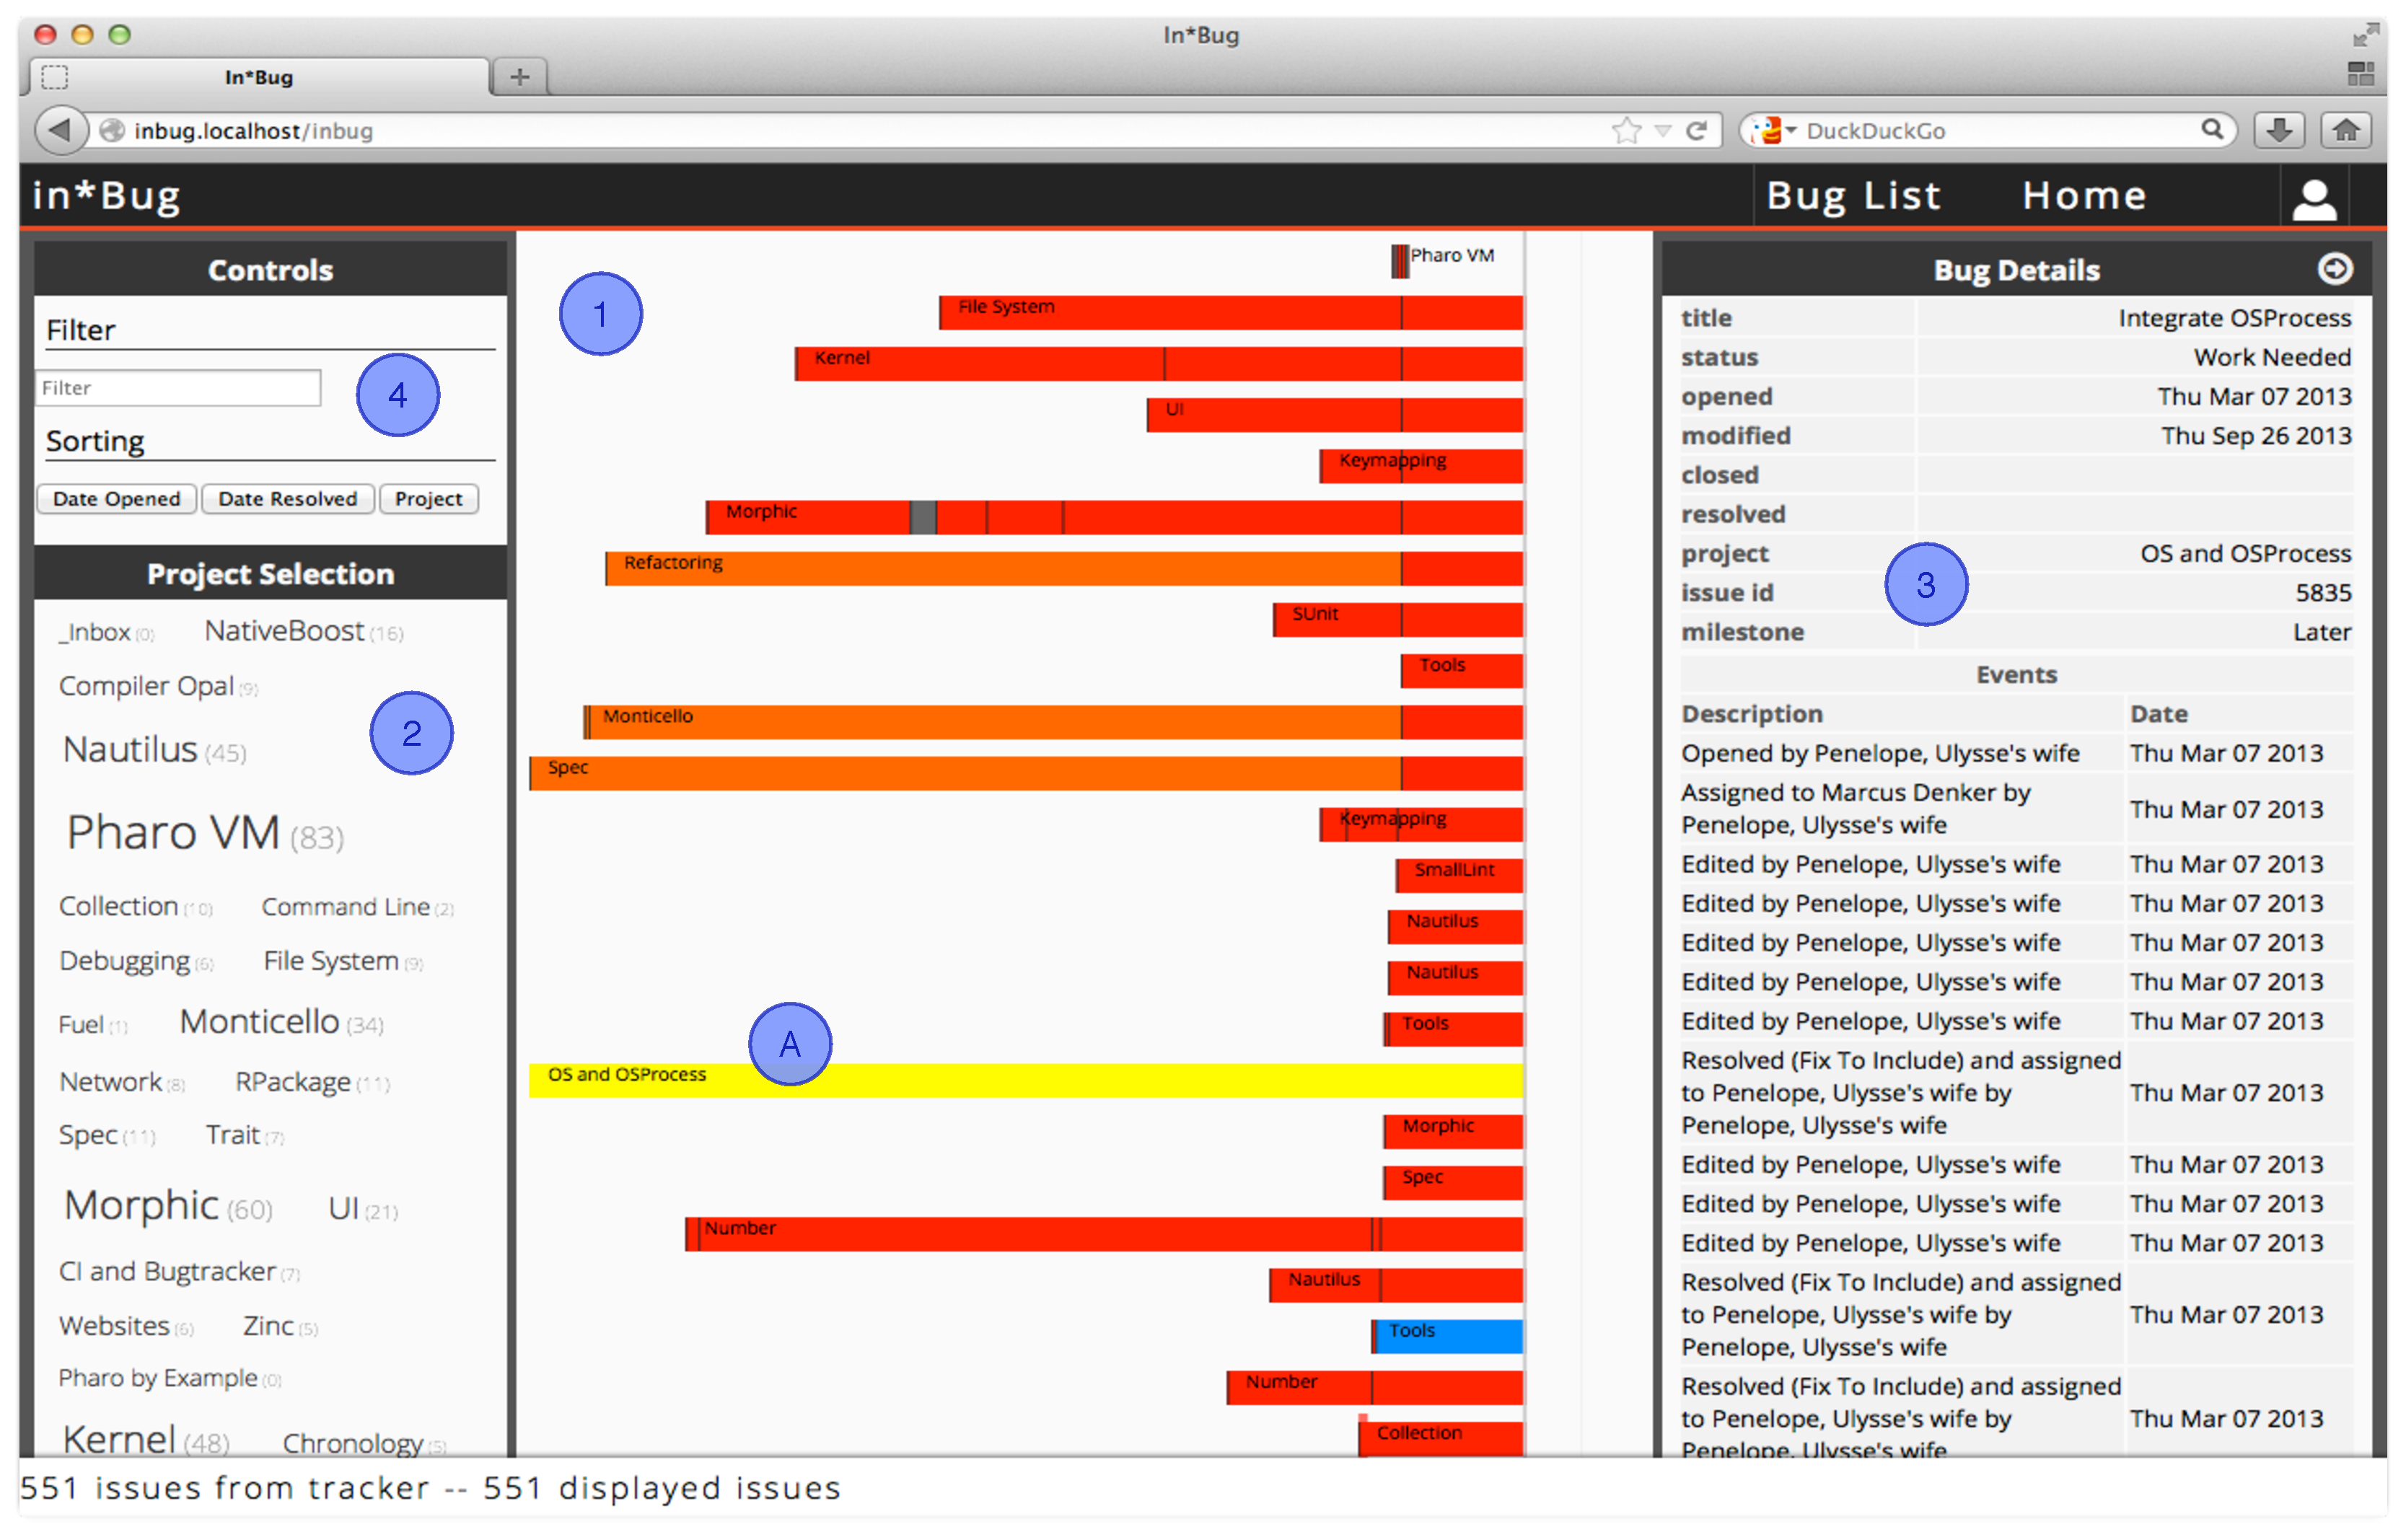
\includegraphics[width=17.4cm]{Images/inbug-list.pdf}
\caption{\ib Main View}
\label{fig-inbug-list}
\end{figure*}

\begin{figure*}
\centering
\includegraphics[width=\linewidth]{Images/inbug-detail.pdf}
\caption{Fine-grained View of a Bug Report}
\label{fig-inbug-details}
\end{figure*}

%%%%%%%%%%%%%%%%%%%%%%%%%%%%%%%%
\section{\ib: an approach for bug visualization}
%%%%%%%%%%%%%%%%%%%%%%%%%%%%%%%%

\ib is a web application built on top of the \textit{Pharo Smalltalk}\footnote{\url{http://www.pharo-project.org}} environment. It uses the \textit{Seaside}\footnote{\url{http://seaside.st}} web framework to provide the data stored in a \textit{MongoDB} database and implements a \textit{RESTful API} to communicate with the client. The client interface is implemented in \textit{JavaScript} using the data manipulation and visualisation library \textit{D3.js}\footnote{\url{http://d3js.org/}}.

\ib is currently targeted at a specific FogBugz repository revolving around the Pharo ecosystem. In \tabref{tab-tracker-summary} we provide a summary of the currently available data.

\begin{table}[ht]
\center
\caption{Summary data of the \textit{Pharo} bug tracker}
\label{tab-tracker-summary}
\begin{tabular}{p{7cm} r}
Number of projects & 46 \\
Number of issues & 8,666 \\
Number of open issues & 613 \\
Total number of events & 79,437 \\
Average events per issue & 9 \\
\end{tabular}
\end{table}

%%%%%%%%%%%%%%%%%%%%%%%%%%%%%%%%%%%%%%%%%%%%%%%%
\subsection{\ib Main View} \label{inbug-list}

\figref{fig-inbug-list} depicts the main user interface, composed of the following panels:

\begin{enumerate}

\item {\bf Bug lifetime panel.} This view depicts the bugs contained in the bug repository, showing their duration (as a horizontal stacked bar chart) and status (using different colors). Each bug tracking system proposes a set of statuses that an issue can acquire. We grouped these statuses into 5 categories, and assigned them the following color codes:

\begin{center}
  {\scriptsize
  \begin{tabular}{p{1.4cm} p{0.1cm} p{1.3cm} | p{1.4cm} p{0.1cm} p{1.2cm} } \hline
  Active & \cellcolor{active} & orange & Work Needed & \cellcolor{work needed} & red \\
  
  Closed & \cellcolor{closed} & gray & Resolved & \cellcolor{resolved} & dark gray \\

  Unknown & \cellcolor{unknown} & light grey & Selected & \cellcolor{yellow} & yellow \\ \hline
  \end{tabular}}
\end{center}



In \figref{fig-inbug-list} one specific bug (marked as A) is under focus. The vertical line to the right indicates the current date.

\item {\bf Project selection panel.} In this panel the user can pick the projects whose bugs she is interested in. All projects are shown as a tag cloud, where the size indicates the number of bugs reported for the project, also indicated with numbers between parentheses close to the name of the projects. 

\item {\bf Details panel.} This panel provides all the information reported about the bug report under focus in the bug lifetime panel. This panel presents both the metadata and the list of events that happened during the lifetime of a bug, including description and date of each event. The metadata is presented as extracted from the bug repository, \eg the opening date, the status or the last modification date. The user can highlight an event to view a popup with the complete description of the event and its comments.

\item {\bf Filter and options panel.} This panel allows the user to sort and filter bugs. The three default sorting criteria order the issues by project, opening date, or date in which the bug has been resolved. The \textit{filter} field offers the possibility to enter either regular expressions or pieces of {\em Smalltalk} code as queries, allowing the users to submit custom made queries to filter bugs.

\item\textbf{Status bar.} This panel shows a quick status of the application. It displays the total number of the bugs in the repository, as for the number of bugs currently selected and visualized.

\end{enumerate}

%%%%%%%%%%%%%%%%%%%%%%%%%%%%%%%%%%%%%%%%%%%%%%%%
\subsection{A Fine-grained View of a Bug Report} \label{inbug-detail}

Aside from the interpretation difficulties that a text based interface presents, \figref{fig-fogbugz-massive} shows that a bug can be composed of a significant number of events. These events are sequential and are triggered by people. They describe the changes in the properties of a bug, such as the opening of a bug, a change of status, the addition of other pieces of information, such as stack traces and screenshots, the assignation to a user who is supposed to fix it, the registration of other people who are interested in that bug, and ultimately also the release (fix) of a bug, who usually comes with a slice of source code. These events are the building blocks of a bug, and visualizing them is the key for its understanding.

\figref{fig-inbug-details} shows our current approach for the detailed depiction of a bug report, composed of three elements that illustrate its different aspects.

\begin{enumerate}[(a)]

\item \label{item-ecg} \textbf{Bug Health} presents the evolution of status of a bug during time. The changes are presented as a line chart that shows the different states in time. The lowest possible value represents the \textit{closed} status, the highest represents the \textit{active} status.

\item \label{item-timeline} \textbf{Bug History} shows a bug report as a timeline composed of its events. If an event changes the status of the bug report, it also changes the color to render the bar. Hovering over a block of the timeline renders the details of the bug report in the details panel. If a new user is involved in the event (\eg a bug is reassigned to someone else), a small circle is rendered at the beginning of the event.
  
\item \label{item-description} \textbf{Bug Event description} is used to display the details of the events. It shows the date and the description of the highlighted event (in yellow in \figref{fig-inbug-details}), such as comments or other pieces of information (\eg stack traces, screenshots) that were added for that event.

\item \textbf{Present time}. The right side of the chart represents the current time. In this case we can observe that the bug is currently still open and its status is ``Work needed''.

\end{enumerate}

%%%%%%%%%%%%%%%%%%%%%%%%%%%%%%%%%%%%%%%%%%%%%%%%%%%%%
\subsection{A Coarse-Grained View of all Bug Reports}

This is the first view, depicted in \figref{fig-inbug-resume}, that is presented to the user, a time-ordered multi-layer stacked chart, which shows how many bug reports were in which status and at which time. 

\begin{figure}[ht]
\centering
\includegraphics[width=\linewidth]{Images/summary-chart.pdf}
\caption{\ib summary view}
\label{fig-inbug-resume}
\end{figure}

Alternatively, the user can also display the various systems to which the bugs belong. This view offers means of interaction to home in on a subset of the bug reports, by using the two sliders at the bottom and on the right. Alternatively, the user can also click on one specific layer, and then jump to the main view depicted in \figref{fig-inbug-list}.

%!TEX root = vissoft2013.tex
% vissoft2013-example


%%%%%%%%%%%%%%%%%%%%%%%%%%%%%%%%
\section{A Usage Example}
%%%%%%%%%%%%%%%%%%%%%%%%%%%%%%%%

We illustrate, through a brief scenario, how \ib can be used to search a bug repository for bugs that need work. We impersonate the user ``Marcus Denker'', who is looking for bugs assigned to him. In the main view of \ib he uses the query engine, composing the \textit{Smalltalk} query shown in \figref{smalltalk-query-one} to find all the opened bugs that are assigned to him.

\begin{figure}[ht]
{\scriptsize
\begin{verbatim}
[ :each | each isActive
and: [ each involvesUser: 'Marcus Denker' ]]
\end{verbatim}
}
\caption{\emph{Smalltalk} query to retrieve the issues assigned to ``Marcus Denker''}
\label{smalltalk-query-one}
\end{figure}

The query returns 461 issues, which he can sort by date or by project. However, these are too many issues to be manually inspected, so he needs to further refine the query. He restricts the research to the reports opened on the 4th April 2013. \figref{smalltalk-query-two} shows the updated query.

\begin{figure}[ht]
{\scriptsize
\begin{verbatim}
[ :each | each isActive
	and: [(each involvesUser: 'Marcus Denker')
	and: [each dateOpened = (Date year: 2013 month: 3 day: 4)
]]]
\end{verbatim}
}
\caption{{\em Smalltalk} query to retrieve the issues assigned to ``Marcus Denker'' opened on April 4 2013}
\label{smalltalk-query-two}
\end{figure}

The query now returns the 13 issues depicted in \figref{fig-inbug-filtered}.

\begin{figure}[ht]
\center
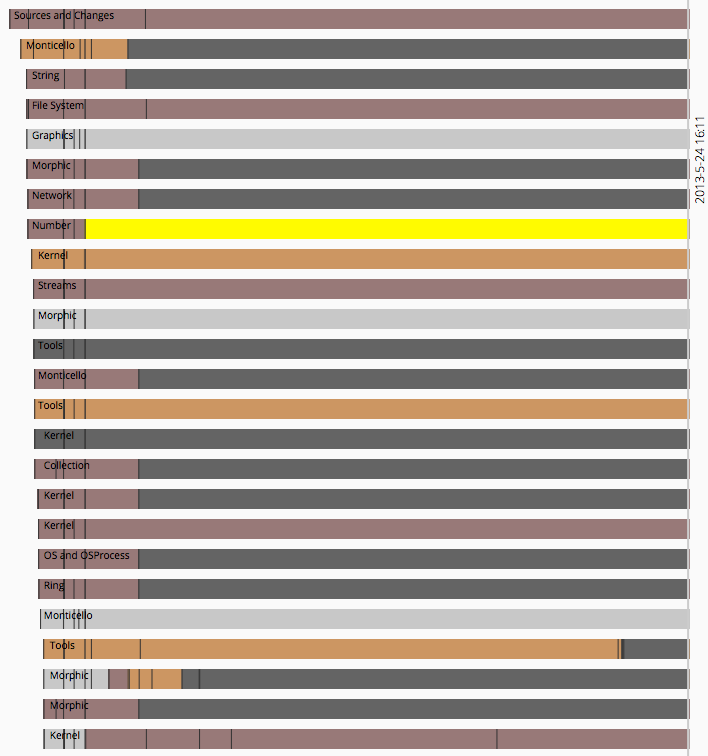
\includegraphics[width=\linewidth]{Images/inbug-filtered.png}
\caption{The result of query in \figref{smalltalk-query-two}}
\label{fig-inbug-filtered}
\end{figure}

Mr. Denker sees that the first bug had some initial activity, but is stalling since then. He uses the fine-grained view to have a complete picture of the issue, depicted in \figref{fig-inbug-reactivated}.

\begin{figure}[ht]
\center
\includegraphics[width=\linewidth]{Images/inbug-reactivated.pdf}
\caption{Detailed view}
\label{fig-inbug-reactivated}
\end{figure}

The view shows that the bug was fixed and then reopened. It is now in status ``Work Needed''. Mr. Denker highlights the last event and sees that the bug was reopened by himself the 22nd of March 2013. Since the issue was marked as ``Resolved'' and then reopened, and it had no activity in a long time, Mr. Denker decides that this is the bug he wants to work on.

With a simple click he is now redirected to the bug's page in the bug tracker.

%!TEX root = vissoft2013.tex
% vissoft2013-related.tex

%%%%%%%%%%%%%%%%%%%%%%
\section{Related Work}
%%%%%%%%%%%%%%%%%%%%%%

Surprisingly, there is only little related work dedicated to the visualization of bug repositories. 

D'Ambros \etal \cite{DAmb2007b} proposed a visualization for bugs as independent entities. Knab \etal \cite{knab2009interactive}\cite{knab2010visual} proposed a set of visualization to ease the process of understanding the data in an issue tracker and find hidden patterns. They also tested their tool in an industrial context. Hora \etal \cite{hora2012bug} proposed a visual exploration of the bug repository, considering bugs as first class entities, and linking them to other software artifacts.

All these approaches focus on retrospective analyses. We believe that while conceptually interesting, there is little practical utility in such a thing, since after all the goal is not to look at bugs, but to actually fix them. This implies that even the most elaborated techniques are of limited actionability, since the bug fixing process takes place in a different space, namely the integrated development environment (IDE). In our case the goal is not to stop at the mere visualization, but then establish a first-class link to the development environment. We envision an environment where going from a specific bug report in \ib to the context where the reported bug can be fixed is a mere mouse click away. Our future efforts will be focused on this goal.

%!TEX root = vissoft2013.tex

%%%%%%%%%%%%%%%%%%%%
\section{Conclusion}
%%%%%%%%%%%%%%%%%%%%

We presented a novel approach to visualize bug repositories, implemented in a visual analytics platform named \ib. \ib currently offers a set of diverse views and interaction means to analyze bug repositories ``in the large'' and then focus on specific bugs ``in the small''. Our short-term goal is to expand the functionalities offered by \ib, refine the visualizations, and then put \ib in ``production mode'', by offering it to the Pharo open-source community.


% use section* for acknowledgement
\section*{Acknowledgements}

We acknowledge the Swiss National Science foundation's support for project 146734 ``HI-SEA''.


\bibliographystyle{IEEEtran}
\bibliography{biblio}


\end{document}


